\documentclass[a4paper,12pt,onecolumn,twoside]{article}
\usepackage{cite}%bibTeX引用
\usepackage{ctex}
\usepackage{hyperref}%加入超链接
\usepackage{comment}
\usepackage{wrapfig}
\usepackage{graphicx}
\usepackage{float} 
\usepackage{amsmath}
\usepackage{amssymb}
\usepackage{geometry}
\geometry{a4paper,scale=0.73}
\usepackage{float}
\usepackage{subfigure} 
\usepackage{enumerate}%\item 需要
\usepackage{tabularx}% \table 
\usepackage{booktabs}% \toprule
\usepackage{tablefootnote}
\usepackage{longtable}
%%带颜色的表格%%
%\usepackage[table]{xcolor}
\usepackage{colortbl}
\definecolor{mygray}{gray}{.9}
\definecolor{mypink}{rgb}{.99,.91,.95}
\definecolor{mycyan}{cmyk}{.3,0,0,0}
%%带颜色的表格%%

%附录代码显示
\usepackage{listings,matlab-prettifier} % MATLAB 美化包
\lstset{
	style=Matlab-editor,
	numbers      = left,
	frame        = single,
}

\usepackage[T1]{fontenc}
\usepackage[utf8]{inputenc}
\usepackage{authblk}

\title{健康规划方案:科学减肥}
\author{学号:20123211~~~~姓名:高雨晴~~~~日期:2022年11月25日}
\date{}
\begin{document}
\maketitle
\tableofcontents
\section{问题重述}
\subsection{引言}
近几十年来,我国居民的生活水平发生了翻天覆地的变化,居民的生活方式也发生了迅速的转变。日益常见的高脂肪、高碳水化合物膳食方式以及体力活动强度的下降,使肥胖率在我国城乡各类人群中迅速上升,成为了一种重要的流行病。联合国世界卫生组织曾颁布人体体重指数(缩写:BMI),其计算方法为体重(单位:kg)除以身高(单位:m)的平方。通常规定BMI在18.5至25为正常,25-30为超重,超过30为肥胖。\par
1989年,中国BMI超重人口只有1.67亿,2009年,这一数字增加到了5.29亿,每天增加4.9万人,年均增长率为10.8\%,甚至超过了同期GDP的增速\cite{niguohua}。肥胖是心脑血管疾病、癌症、糖尿病等慢性疾病的重要诱因,被世界卫生组织列为威胁人类健康的十大疾病之一,当然,越来越多的人逐渐意识到了肥胖对健康的危害,开始注意饮食习惯,积极参与户外运动。在大学生群体中,减肥不失为一种潮流,不过更多的人体重远未达到威胁健康的程度,而是为了更加美观的外形而减肥。\par
\begin{figure}[H]
	\centering
	
\includegraphics[width=0.8\linewidth]{res/shenteng.jpg}
	\caption{肥胖对一个人气质的影响往往是毁灭性的(图片来自网络)}
\end{figure}
有需求就有市场,有市场往往就有骗局。大量的减肥机构和减肥商品出现,然而事实上,很多减肥机构提供的服务和减肥产品要么是“智商税”,要么是安慰剂,如“推拿减肥法”、“减肥果冻”等。这些服务和产品忽略了减肥最基本的原理,即减重的多少取决于能量摄入和能量消耗产生的缺口。本文将基于此原理构建数学模型,以虚拟人物小高为例,制定合理的减肥方案,并对减肥方案进行探讨和分析。
\subsection{问题背景与问题提出}
\subsection*{问题背景}\label{background}
\paragraph{个人信息~}现收集到小高的个人信息如表\ref{personalinfo}所示。
\begin{table}[H]\label{personalinfo}
	\centering
	\caption{小高的个人信息}
	\begin{tabular}{c|c|c|c} 
		\hline\hline
		姓名 & 高某某(小高)& 身高 & 163 cm  \\\hline
		性别 & 女           & 体重 & 65 kg   \\\hline
		年龄 & 21 岁         & 目标体重 & 50 kg\\\hline
        每日摄入能量 & 约2000 kcal & 每日饮食计划支出 & 30 元\\\hline
		\hline
	\end{tabular}
\end{table}
\paragraph{食物信息~}现收集到小高爱吃的几种菜品信息如表\ref{foodinfo}所示。
\begin{table}[H]\label{foodinfo}
	\centering
	\caption{小高爱吃的食物信息}
	\begin{tabular}{c|c|c|c} 
		\hline\hline
		菜名 & 价格(人民币/100g)& 热量\tablefootnote{数据来自\url{https://www.boohee.com/food}}(kcal/100g)& 喜爱程度(0-5)   \\\hline
		日本豆腐肥牛 & 3.25 & 151 & 4.7  \\\hline
		烧鸭饭 & 2.2  & 157 & 3.9\\\hline
		照烧鸡排饭 & 3 & 172 & 4.9\\\hline
		双拼炸鸡饭 & 2.8 & 183 & 3.4\\\hline
		兰州拉面 & 3 & 136 & 3.5\\\hline
		香肉拌饭 & 2.75 & 257 & 4.3\\\hline
		烤鸭 & 5 & 379 & 4.0\\\hline
		五谷渔粉& 3 & 169 & 3.4\\\hline
		焦溜肥肠& 3.25 & 176 & 3.5 \\\hline
		轻食沙拉(外卖)& 8.8 & 90 & 5.0 \\\hline  
		\hline
	\end{tabular}
\end{table}
%其中我们规定,当连续两天吃同一种菜品时,喜爱程度-1。每一天作出决策时,小高不会购买喜爱程度小于0的菜品。
\paragraph{运动信息~}小高几乎任何常见的体育项目都不会,且平时不运动,故只展示三种常见的运动,如表\ref{sportsinfo}所示。
\begin{table}[H]\label{sportsinfo}
	\centering
	\caption{小高能接受的运动信息}
	\begin{tabular}{c|c} 
		\hline\hline
		运动名称 & 消耗热量\tablefootnote{数据来自网络.}(kcal/h$\cdot$kg) \\\hline
		散步 & 1.7 \\\hline
		快走 & 5.8 \\\hline
		慢跑 & 7.0 \\\hline
		\hline
	\end{tabular}
\end{table}
%一周之中,当连续两天做同一种运动时,抗拒程度+1。每一天作出决策时,小高会选择做抗拒程度最低的运动。
\subsection*{问题提出}安排一个两阶段计划,使得小高能够以相对少的时间和金钱成本达到减肥目标。
\paragraph{第一阶段~}若要求在不运动的情况下每周减肥0.25kg,每周吸收热量逐渐减少直至达到下限,试安排第一阶段的减肥计划。
\paragraph{第二阶段~}若要加快进程,第二阶段增加运动,试安排第二阶段的减肥计划。
\paragraph{第三阶段~}若达到目标后需要维持体重,试给出方案。
\section{问题分析}
减肥最基本的原理是:减去的体重所转化的热量等于消耗的热量与摄入的热量之差。则可以根据这项原则建立差分方程模型,反映每周结束时的体重与每周开始时体重的关系。通过该模型,我们可以进一步地通过已计划的要求(每周需要减去多少kg体重、目标体重是多少等),获得我们制定计划所需的一些数值(如每周需要摄入多少热量等)。而至于计划的进一步制定,我们可以从消耗的热量与摄入的热量两方面着手,分开分析。\par 
人类摄入的热量只来源于食物。在第一阶段,由于我们已知每周需要减去的体重,因此不难通过差分方程模型求出每周需要摄入的热量。由此,我们可以对食物的各项指标(热量、价格、偏爱)进行分析,通过线性规划的方法作出决策。\par 
而人类消耗的热量可以分划为很多具体的类别。本问题中,为了简化模型,我们认为人体消耗的热量只归为两类:运动消耗和身体代谢消耗。根据假设,身体代谢消耗是和体重线性相关的,因此我们可以根据体重稳定时的差分方程来确定这一线性系数,确定后便用于整个模型(当然这是不够合理的,进一步的讨论见\nameref{choosebeta})。由于代谢消耗热量是我们无法人为控制的,因此剩下的热量窗口,我们需要通过安排运动计划来填补。
\section{模型假设与符号说明}
\subsection*{模型假设}
\paragraph{假设一~}每摄入8000kcal会增加1kg体重。
\paragraph{假设二~}代谢和运动引起的体重减少正比于体重。
\paragraph{假设三~}为简化模型,小高每天只吃一种食物(不考虑早中晚饭的区别),每天只选择一种运动方式。
\paragraph{假设四~}为了安全与健康,每周体重减少不宜超过1.5kg,每周吸收热量不要小于10000kcal.
\subsection*{定义与符号说明}
\begin{longtable}{cc}
		\toprule
		符号 & 定义与说明说明(单位)\\\hline
		$W(k)$      & 第$k$周体重(kg) \\
		$Cal_{in}$  & 热量摄入(kcal) \\
		$Cal_{out}$ & 热量消耗(kcal) \\
		$\alpha$    & 热量-体重转换系数\\
		$\beta$     & 代谢消耗系数\\
		$R_i$       & 食物种类\\
		$x_{i}$     & 第$i$种食物的份数($\cdot$ 100g)\\
		\hline
		\hline
		符号 & 定义与说明说明(单位)\\\hline
		$C$         & 周计划摄入热量(kcal)\\
		$e_i$       & 每份$R_i$所含热量(kcal)\\
		$p_i$       & 每份$R_i$价格(元)\\
		$h_i$       & 每份$R_i$满足度\\
		$\gamma$    & 每小时每千克体重消耗热量(kcal)\\
		$t$         & 每周运动时间(h)\\
		$\beta^{\prime}$ & 热量消耗系数\\\bottomrule
\end{longtable}
\section{模型的建立和求解}
\subsection{准备工作:摄入与消耗\label{sensitivity:beta}}
我们用$W(k)$表示小高第$k$周的体重,$Cal_{in}$和$Cal_{out}$分别代表热量的摄入和消耗。由假设一,定义热量体重转换系数$\alpha=\frac{1}{8000}$(kg/kcal)。于是第$k+1$周的体重为
\begin{equation}\label{eqmain}
	W(k+1)=W(k)+\alpha(Cal_{in}-Cal_{out})
\end{equation}
其中每周热量的摄入全部来自食物。每周能量的消耗分为两部分:运动带来的能量消耗$Cal_{sports}$以及新陈代谢的基础消耗$Cal_{meta}$。定义代谢消耗系数$\beta$,由假设二有
\begin{equation}
	Cal_{meta}(k)=\beta W(k)
\end{equation}
假设小高每周摄入量为$Cal_{in0}$,消耗量为$Cal_{out0}$时体重维持在$W_{0}$不变,则根据
\begin{equation}
	W_{0}=W_{0}+\alpha(Cal_{in0}-Cal_{out0})
\end{equation}
根据\nameref{background},小高平时不运动,因此$Cal_{out0}=\beta W_{0}$,由此得到$\beta$的计算公式
\begin{equation}\label{def:beta}
	\beta=\frac{\alpha Cal_{in0}}{W_{0}}
\end{equation}
将表\ref{personalinfo}中数据代入计算,最后得到小高的代谢系数$\beta=0.024$.
\subsection{第一阶段:少吃不动}
\subsubsection{总计划}
本计划第一阶段的目标是:在不运动的情况下,体重每周减少0.25kg,直至$Cal_{in}(k)$减至下限10000kcal。设第$k$周结束时,摄入的热量为$Cal_{in}(k)$.则根据关系$W(k)-W(k+1)=0.25$和(\ref{eqmain})有
\begin{equation}
	Cal_{in}(k+1)=\frac{\beta W(k)-0.25}{\alpha}
\end{equation}
又因为$W(k)=W_{0}-0.25k$,上式可写为
\begin{equation}\label{sensi:1}
	Cal_{in}(k+1)=\frac{\beta W_{0}}{\alpha}-\frac{0.25+\beta k}{\alpha}
\end{equation}
当$Cal_{in}(k+1)\leq 10000$时停止迭代,经计算\footnote{计算过程见附录“phase1.m”}有$k=3$. 即第一阶段耗时3周,每周减重0.25kg,在第4周结束后,小高的体重为64.25kg.
\subsubsection{饮食计划:多目标线性规划方法}在总计划中,我们得到了第一阶段每周小高需要摄入的能量总值如表\ref{phase1calin}所示,接下来我们需要结合小高的个人喜好以及经济实力,为小高制定一个易于坚持的食谱。根据表\ref{foodinfo},建立一多目标线性规划模型。%这部分真你妈难,等过两天学学数学规划再写
%吗的决策变量是二维的->笨,改成一维就好啦
\begin{table}[H]\label{phase1calin}
	\centering
	\caption{第一阶段每周摄入热量}
	\begin{tabular}{cc} 
		\toprule
		周数 & 计划摄入热量(kcal)\\\hline
		第一周 & 10480 \\
		第二周 & 10240 \\
		第三周 & 10000 \\\bottomrule
	\end{tabular}
\end{table}
称100g食物为"一份"。根据成年女性通常的食量,推荐小高每日摄入食物的总重量不超过1kg。每日从表\ref{phase1calin}中自上而下地选择第$i$种食物$R_{i}$若干份作为一天的饮食,记作$x_{i}$,其中$i=1,2,...,10.~$在本周计划摄入热量$C$已经确定的情况下,出于健康考虑,我们不妨设每天摄入的热量一样多,即每天的热量摄入均为$C/7$。我们可以构造以下的目标函数:
\paragraph{$\bullet$~价格目标函数~}记每份$R_{i}$中含有热量$e_{i}$,构成热量列向量\textbf{E}. 价格为$p_{i}$,构成价格列向量\textbf{P}. 则价格目标函数为:
\begin{align*}
	&\min \quad z_1= \sum_{i=1}^{10}  x_{i}p_{i} \\
	s.t.& \left\{ \begin{array}{r@{\quad}l@{}l@{\quad}l}
		& \sum\limits_{i=1}^{10} x_{i}e_{i}=C/7\\
		&\sum\limits_{i=1}^{10} x_{i}p_{i}\le 30\\
		&\sum\limits_{i=1}^{10} x_{i}\le 10\\
		& x_{i} \ge 0,  &i=1,2,...,10.
	\end{array}\right.
\end{align*}
\paragraph{$\bullet$~满足度目标函数~}我们将喜爱度量化为每份$R_{i}$带给小高的满足度$h_{i}$,构成满足度列向量\textbf{H}. 则满足度目标函数为:
\begin{align*}
	&\max \quad z_2= \sum_{i=1}^{10}  x_{i}h_{i} \\
	s.t.& \left\{ \begin{array}{r@{\quad}l@{}l@{\quad}l}
		& \sum\limits_{i=1}^{10} x_{ij}e_{i}=C/7\\
		&\sum\limits_{i=1}^{10} x_{i}p_{i}\le 30\\
		&\sum\limits_{i=1}^{10} x_{i}\le 10\\
		& x_{i} \ge 0,  &i=1,2,...,10.
	\end{array}\right.
\end{align*}
解多目标线性规划问题通常的方法有线性加权法、极大极小法、理想点法等。在本问题中,我们尝试使用线性加权法求解。
\paragraph{线性加权法~}该方法将目标函数通过效用函数建立相关关系,即为不同的目标函数赋权,从而使多目标规划问题转化为单目标规划问题。权值的确定有很多种,例如专家打分法、容限法和加权因子分解法等。由于该饮食计划是为小高制定,故我们使用“专家打分法”是最合适的:在小高看来,少花钱和吃好的重要性可以三七开,则我们可以为两个目标函数分别赋权$\omega_{1}=0.3,\omega_{2}=0.7$. 在目标函数按权加和之前,我们需要消除两个指标\textbf{P}和\textbf{H}的量纲影响,即进行标准化。一个比较常用的标准化方法是“min-max标准化法”,以\textbf{P}为例,对其中任意元素$p_i$,有
\begin{equation}
	p_i^\star=\frac{p_i-p_{min}}{p_{max}-p_{min}}
\end{equation}
于是问题转化为:
\begin{align*}
	&\min \quad z= 0.3\sum_{i=1}^{10}  x_{i}p_{i}^\star-0.7\sum_{i=1}^{10}  x_{i}h_{i}^\star \\
	s.t.& \left\{ \begin{array}{r@{\quad}l@{}l@{\quad}l}
		& \sum\limits_{i=1}^{10} x_{i}e_{i}=C/7\\
		&\sum\limits_{i=1}^{10} x_{i}p_{i}\le 30\\
		&\sum\limits_{i=1}^{10} x_{i}\le 10\\
		& x_{i} \ge 0,  &i=1,2,...,10.
	\end{array}\right.
\end{align*}
经计算\footnote{计算过程见附录“foodchoice.m”},在第一周至第三周为小高设计的食谱如下表所示。
\begin{table}[H]
	\centering
	\caption{第一至三周每天的饮食计划}
	\begin{tabular}{c|c|c} 
		\hline
		周数 & 计划热量(kcal) & 饮食计划  \\\hline
		Ⅰ & 10480 & 50.7~g~日本豆腐肥牛,800~g~照烧鸡排饭,49.4~g~轻食沙拉 \\\hline
		Ⅱ & 10240 & 21.7~g~日本豆腐肥牛,800~g~照烧鸡排饭,60.2~g~轻食沙拉 \\\hline
		Ⅲ & 10000 & 793.9~g~照烧鸡排饭,70.3~g~轻食沙拉 \\\hline
	\end{tabular}
\end{table}

\subsection{第二阶段:少吃多动}\label{sensi:phase2}
本计划第二阶段的目标是:加快减重速度,每周保持$Cal_{in}=10000~\text{kcal}$(事实上,在上一节的计算中,第三周的热量摄入恰巧是10000 kcal),配合运动,直至体重减至50kg。假设每小时每千克体重消耗的热量为$\gamma$(单位:kcal),每周运动的时间为$t$(单位:h),则根据假设二,有
\begin{equation}
	Cal_{sports}(k)=\alpha\gamma t\cdot W(k)
\end{equation}
不妨定义热量消耗系数$\beta^{\prime}=\beta+\alpha\gamma t. $根据(\ref{eqmain})有递推关系
\begin{equation}\label{eq1}
	W(k+1)=(1-\beta^{\prime})W(k)+\alpha Cal_{in}
\end{equation}
由式(\ref{eq1})可推出第$k+n$周和第$k$周体重的关系为
\begin{equation}\label{sensi:2}
	\begin{aligned}
		W(k+n)&=(1-\beta^{\prime})^{n}W(k)+\alpha Cal_{in}[1+(1-\beta^{\prime})+\cdots+(1-\beta^{\prime})^{n-1}]\\
		&=(1-\beta^{\prime})^{n}[W(k)-\frac{\alpha Cal_{in}}{\beta^{\prime}}]+\frac{\alpha Cal_{in}}{\beta^{\prime}}
	\end{aligned}
\end{equation}
取$\gamma t=72$,这相当于每周跑步10.3小时或快走12.4小时,或散步42.4小时。则$\beta^{\prime}=0.024+0.009=0.033$.令$W(k+n)=50$,经计算\footnote{计算过程见附录“phase2.m”}有$n=23.1642$,即第二阶段耗时23周。

\subsection{维持体重:多动才能多吃}
达到目标体重后,为了使小高能够保持在这个体重不变,她必须相对之前作出改变——要么比之前吃得少,要么比之前运动量多。根据小高提供的信息,她没有运动的习惯,想必在我们的减肥计划执行过程中,大量的运动也为她带来了极大的痛苦。那么,如果小高在减肥成功后再也不运动了,我们可以根据公式
\begin{equation}
	W(k+1)=W(k)+\alpha Cal_{in}-\beta^{\prime}W(k)
\end{equation}
来计算小高此后每周能够摄入的热量$Cal_{in}.$ 由于此时的任务是维持体重,故$W(k+1)=W(k)=W(=50\text{kg}).$ 于是有
\begin{equation}
	Cal_{in}=\frac{\beta^{\prime}\cdot W}{\alpha}
\end{equation}
若不运动,则$\beta^{\prime}=\beta=0.024$,$Cal_{in}=9600$ kcal. 按天计算,则小高每天大约只能吃1371 kcal,换算成小高爱吃的烤鸭,则每天只能吃360 g左右。这显然是令人难以接受的,并且也不符合假设四的要求,因此我们不推荐小高在减肥成功后完全不运动。 \par
若保持第二阶段的运动量,则$\beta^{\prime}=0.033$,$Cal_{in}=13200$ kcal. 按天计算,小高每天可以吃大约1885 kcal,这是符合一个成年女性的正常摄入量的。当然,小高也可以根据自身意愿合理安排运动,按照我们的模型灵活调节运动和摄入,以达到维持体重的目的。
\section{模型评价与改进}
\subsection{模型评价}
\paragraph{模型的优点}差分方程模型在首先保证了符合科学规律的情况下,使各阶段的求解易于计算,较准确地模拟了减肥的过程。
\paragraph{模型的缺点}模型的众多假设事实上是过于简化的。并且,以食谱规划为例,我们在考虑为减肥中的人配餐时,除了热量之外,也要考虑其各类营养素含量,因为如果长时间无法全面摄入人体所需营养元素,可能会对身体造成伤害,进而影响身体的代谢,这会大大影响模型的稳定性。而模型本身对代谢系数是敏感的,我们将在下一节详细讨论这一点。
\subsection{模型的改进}
\subsubsection{灵敏性分析:代谢系数的选择}\label{choosebeta}
在\nameref{sensitivity:beta}中,我们定义了代谢系数$\beta$,并且有计算公式(\ref{def:beta}). 但该计算公式是非常粗糙的,因为人体的代谢会受到很多因素影响,而并非只与体重成正比。举个简单的例子,同样身高体重的相扑选手和每天抱着薯片在电视机前躺一天的肥宅,他们的代谢水平是天差地别的。而同一个人哪怕一辈子都保持相同的身材,他在青壮年时期的代谢水平和老年时期的代谢水平也相差显著。
\begin{figure}[H]
	\centering
	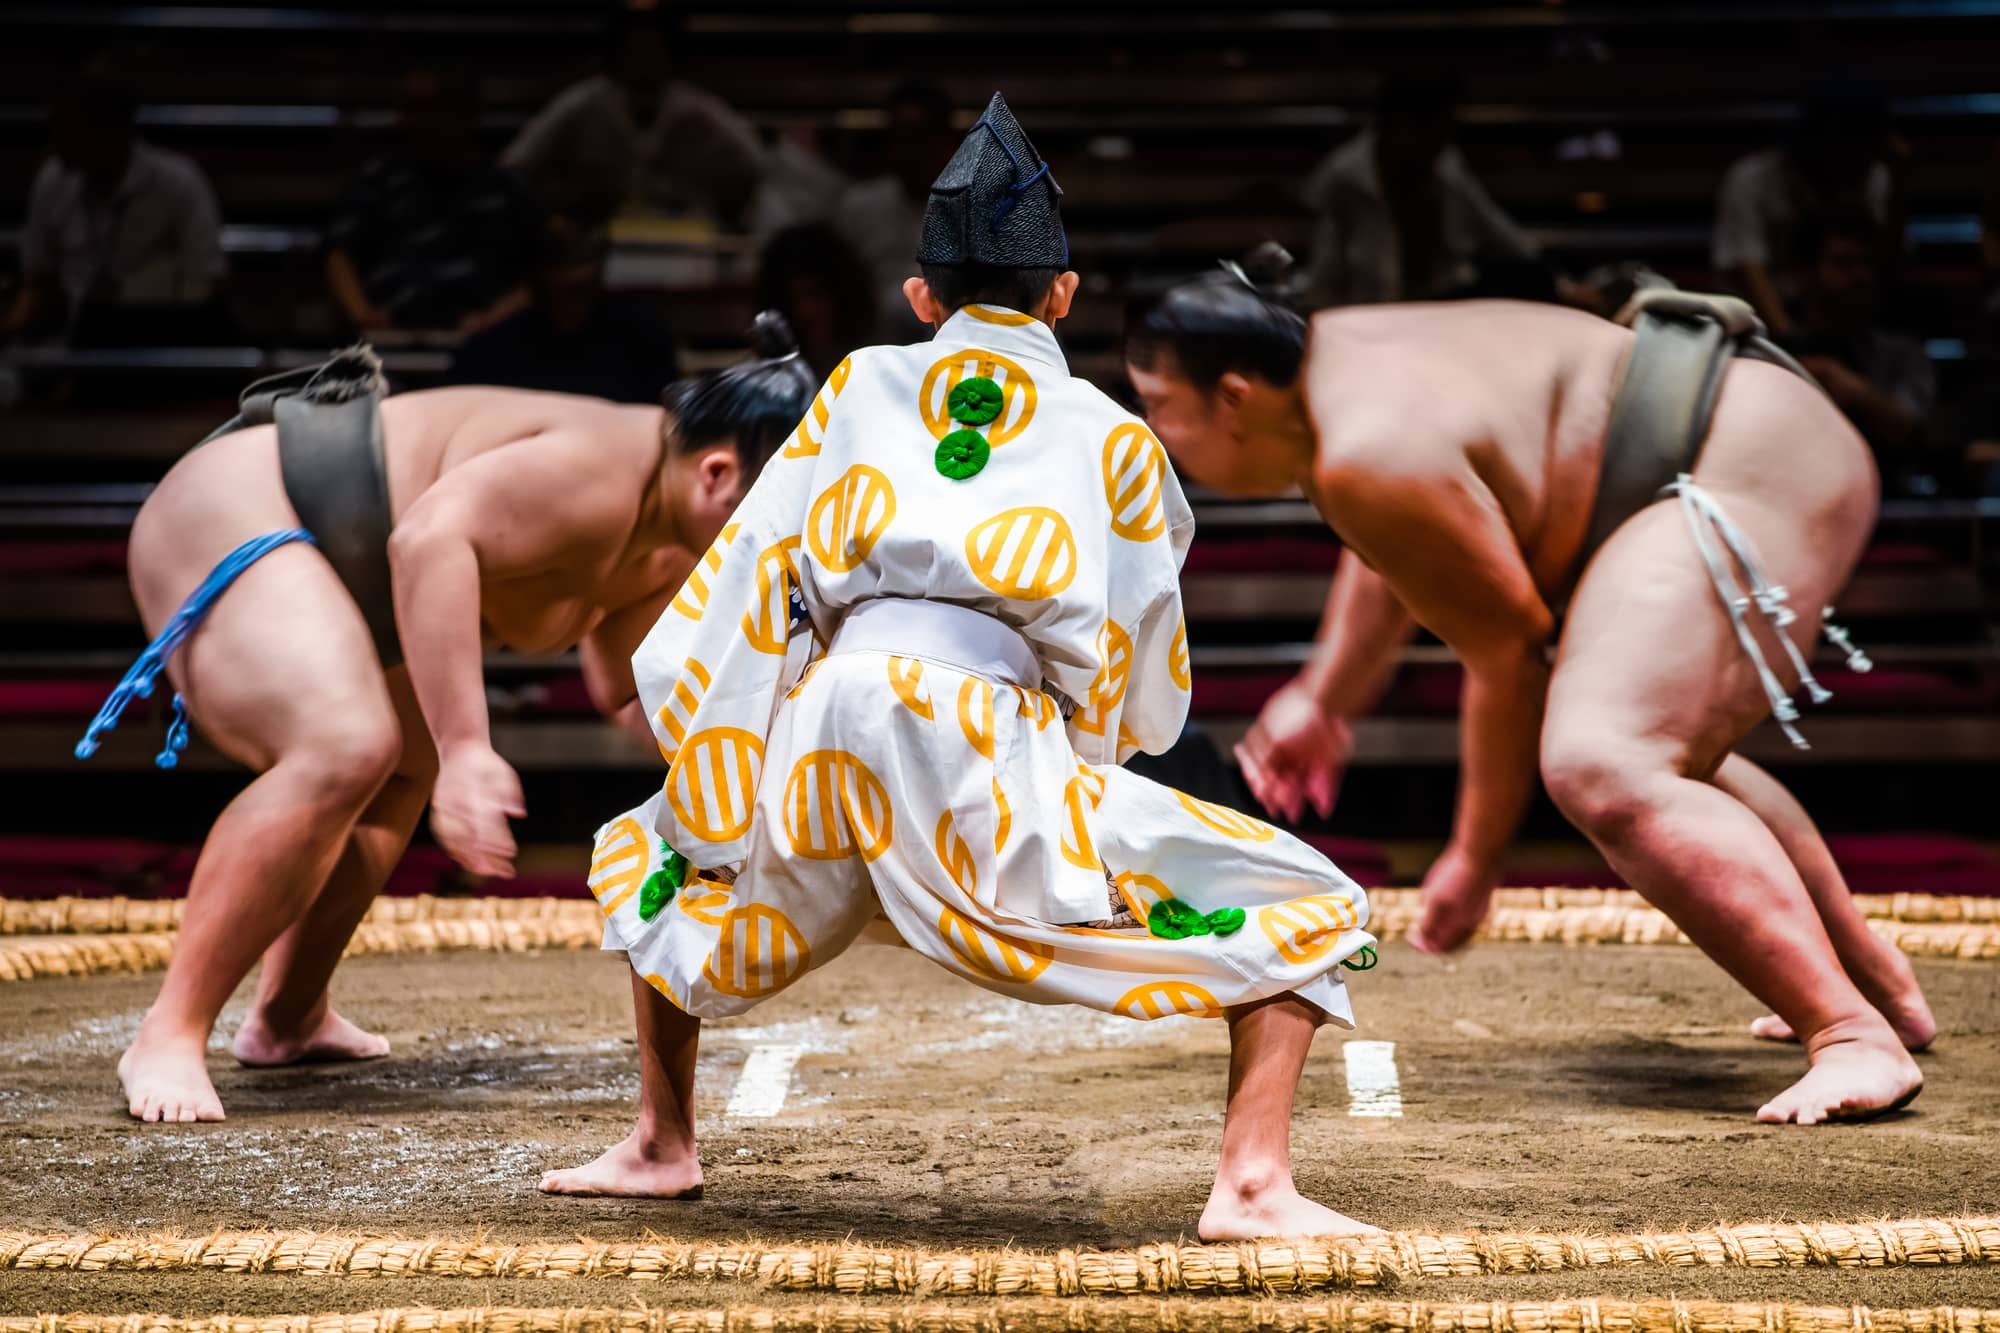
\includegraphics[width=0.8\linewidth]{res/sumo.jpg}
	\caption{相扑运动员每天要摄入18500-19000千卡的热量,比小高减肥前一周吃得都多\protect\footnotemark}
\end{figure}
\footnotetext{图片来自\url{https://thegate12.com/cn/article/6}}
而我们在建立模型时使用的许多计算公式均对$\beta$的取值敏感,如式(\ref{sensi:1})和式(\ref{sensi:2})。我们以第二阶段为例进行灵敏性分析。在\nameref{sensi:phase2}中我们使$\beta^{\prime}$从0.033以0.001步长增长至0.044,共变化33\%. 第二阶段需要的天数n对应的变化如图所示。
\begin{figure}[H]
	\centering
	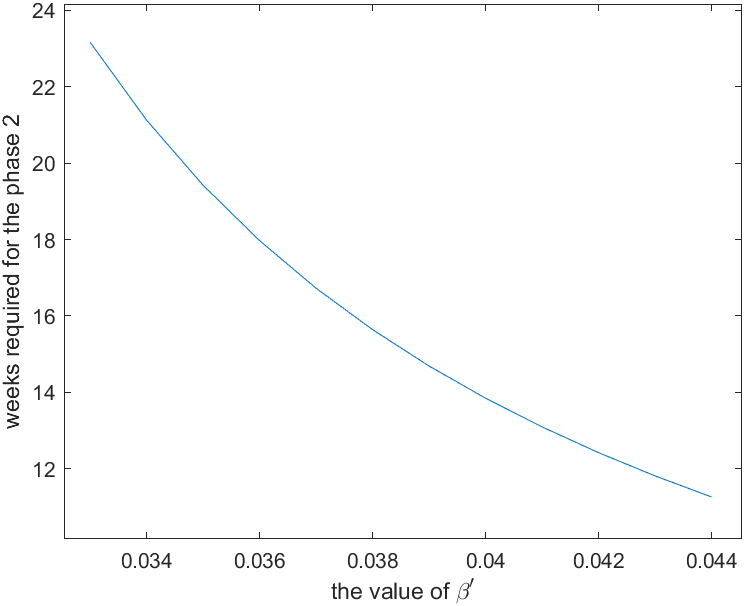
\includegraphics[width=0.7\linewidth]{res/sensitivity.png}
	\caption{第二阶段天数n随$\beta^{\prime}$的变化}
\end{figure}
由图可以直观地看出,当代谢系数$\beta^{\prime}$小范围变化时,第二阶段所需天数便发生明显变化,当其变化33\%时,第二阶段所需天数几乎缩短至原来的一半。因此,对模型的改进可以从代谢系数着手,通过更加科学的计算方式来确定代谢的消耗。
\subsubsection{模型改进:代谢热量的另一种计算方式}
根据Harris和Benedict的研究\cite{henry2005basal},成年女性每日的新陈代谢导致的能量消耗$BMR$(单位:kcal)可以由下式计算得出:
\begin{equation}\label{bmr}
	BMR(k)=665.0955+9.5634W(k)+1.8496H-4.6756A
\end{equation}
其中,%$W(k)$为第$k$周体重,单位kg。
$H$为身高,单位cm。$A$为年龄,单位岁。由(\ref{bmr})可得
\begin{equation}
	Cal_{meta}(k)=7\times BMR(k)
\end{equation}
代入表\ref{personalinfo}中数据,可以计算出小高在减肥前的每日新陈代谢能量消耗是1490 kcal. 小高在减肥过程中体重逐渐降低,$BMR$也随之线性变化,这也是符合假设二的,但由于其考虑了性别、年龄、身高等因素的影响,比起前文的定义更加易于解释。我们再编写程序\footnote{见附录“sensitivity2.m”}测试引入$BMR$后模型的敏感性。根据公式(\ref{eqmain}),改进后第二阶段的体重计算公式为
\begin{equation}
	W(k+1)=W(k)+\alpha(Cal_{in}-7\cdot(868.3927+9.5634\theta W(k))-\gamma tW(k))
\end{equation}
其中,$BMR$中的身高、年龄变量已代入数据计算,$\theta$是变化系数。由于在上一节中,我们使$\beta^{\prime}$总共变化了33\%,为了便于对照,我们使$\theta$从100\%以3\%的步长变化至133\%,其余变量取值均与上一节相同,最后考察第二阶段减肥所需时间如图所示。
\begin{figure}[H]
	\centering
	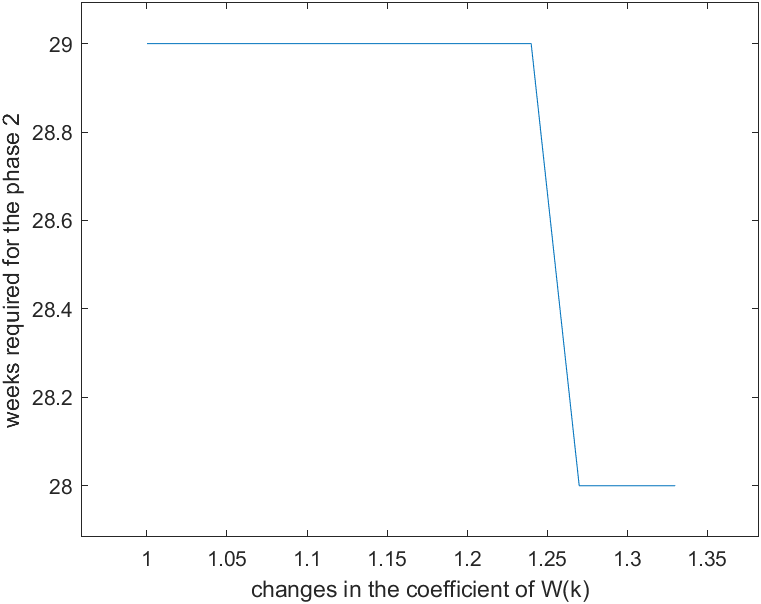
\includegraphics[width=0.7\linewidth]{res/sensitivity2.png}
	\caption{第二阶段天数n随$BMR$中体重系数的变化}
\end{figure}
可见在引入$BMR$后,系数小范围变化时,第二阶段所需天数没有发生改变,而系数变化33\%,第二阶段所需天数也只减少了1天。因此我们可以认为,使用$BMR$改进模型能够使模型的稳定性更好。
\addcontentsline{toc}{section}{参考文献}
\bibliographystyle{IEEEtran}
\bibliography{cite}
\section{附录:\textbf{MATLAB}代码}
\lstinputlisting[caption={\bf phase1.m},]{code/phase1.m}
\lstinputlisting[caption={\bf foodchoice.m},]{code/foodchoice.m}
\lstinputlisting[caption={\bf phase2.m},]{code/phase2.m}
\lstinputlisting[caption={\bf sensitivity.m},]{code/sensitivity.m}
\lstinputlisting[caption={\bf sensitivity2.m},]{code/sensitivity2.m}
\end{document}
